\documentclass[11pt,letterpaper]{article}

% Load some basic packages that are useful to have
% and that should be part of any LaTeX installation.
%
% be able to include figures
\usepackage{graphicx}
% get nice colors
\usepackage{xcolor}

% change default font to Palatino (looks nicer!)
\usepackage[latin1]{inputenc}
\usepackage{mathpazo}
\usepackage[T1]{fontenc}
% load some useful math symbols/fonts
\usepackage{latexsym,amsfonts,amsmath,amssymb}

% comfort package to easily set margins
\usepackage[top=1in, bottom=1in, left=1in, right=1in]{geometry}
\usepackage{hyperref}
\usepackage[all]{hypcap}
% control some spacings
%
% spacing after a paragraph\begin{figure}[bth]
\setlength{\parskip}{.15cm}
% indentation at the top of a new paragraph
\setlength{\parindent}{0.0cm}

\begin{document}

\begin{center}
\Large
Ay190 -- Final: Project 8 Orbital Integrations \\
David Vartanyan\\
Date: \today
\end{center}

\section{Introduction}
We solve the 2-body and 3-body systems using the Earth-Sun and Earth-Sun-Moon as our canonical configuration.

The code we develop is applicable to any N-body configuration and it uses our earlier work on Worksheet 13, which is available on \url{https://github.com/dvartany/ay190/tree/master/ws13}\label{tex:1}.

The reader should keep in mind two things when running the code.

First - since the latter half of the code becomes heavy on processor power (explained below), I aimed to streamline my code. As a result, I used the energy and acceleration functions written by Roland Haas and posted by Michael Weastwood in the solutions section \url{https://github.com/mweastwood/Ay190Solutions/blob/master/ws13/ws13_nbody.py}, which runs significantly faster than anything we wrote. The interested reader can compare its runtime with my ws13 link above \ref{tex:1} or with Mee's at \url{https://github.com/cwongura/Ay190_Mee/blob/master/Project/Project_Lib.py}.

Second - the initial code was written independently by me and Mee. Only later did we collaborate and compare. The result is a stitched code where the 2-body project code is distinct whereas the 3-body code overlaps between our work. Thus, while our Integrator.py and Project\_Library.py files are (largely) different, we use the same code to explore the Kozai mechanism.

\section{Readme}
Below we provide a basic map to the final repository. The RK4 and leapfrog integrators are in Integrator.py. The energy, earth-moon distance, and eccentricity functions are in Project\_Lib.py.\\newline

The code up to but not including the Kozai mechanism are in ay190final.py, which calls on the previous libraries. Structurally, this code is nearly identical to the template presented for Worksheet 13. It calls on three different data files. Sun\_earth.asc contains positions and velocities in 3-dimensions for these two bodies. It has the special property that it is normalized so that the sun is slightly off-focus and thus the center of mass (which is not the sun) remains stationary thought the sun may move. Sun\_earthecc.asc contains the same data but for Earth at an eccentricity of $0.5$. Semoon.asc contains the same kinematic data for the sun, earth, moon 3-body system. Here, the sun is at the origin and is not offset as before.\\newline

This code concludes with a series of plots, including the moon orbital radius, 3-D orbits, energy errors for different integrators.\\newline

ecc.py is usd to plot eccentricity as a function of inclination to illustrate the Kozai mechanism. It is identical to Mee's Figure\_Kozai\_MaxEcc.py

The reference papers used are \href{http://iopscience.iop.org/0004-637X/535/1/385/pdf/40691.web.pdf}{Ford et al 2010: Secular Evolution of Hierarchical Triple Star Systems} and \href{http://adsabs.harvard.edu/cgi-bin/bib_query?1962AJ.....67..591K}{Kozai 1962: Secular Perturbations of Asteroids with High Inclination and Eccentricity}.

\section{Integrators:Leapfrog and RK4}

We explore error propagation using two different integrators: Leapfrog and RK4.
A description of RK4 is available in the class notes online; we omit repeating it below. Since the leapfrog method is incorrect on the class notes, we have summarized it below.

\begin{equation}
x_{n+1}=x_n+v+n\Delta t+\frac{1}{2} \Delta t^2
\end{equation}
\begin{equation}
v_{n+1}=v_n+\frac{1}{2}(a_n+a_{n+1})\Delta t
\end{equation}

The leapfrog is favorable over RK4 because it is symplectic - it convserves energy. The leapfrog method uses information at the previous and current timestep, whereas RK4 depends only on the previous.

As we can see in Figure ~\ref{fig:1} plotting energy error over the first 80 years for the Sun-Earth Orbit, RK4 accumulates error, leapfrog doesn't but rather oscillates. For the remainder of the problem we will be using RK4 integration unless otherwise specified for the sake of computing speed. 

\section{Resolution}
We explore how modifying the resolution will affect error. We change Nsteps in our code to the values indicated in the linked figures.

We compare a low resolution RK4 integrator with only $1000$ steps in ~\ref{fig:2} to a high resolution RK4 integrator with $50000$ steps in ~\ref{fig:3}

\section{Earth-Sun eccentricity}
Next we add an eccentricity of $0.5$ to Earth's orbit. RK4 Error increases by several orders as we can see by comparing a circular orbit, Figure ~\ref{fig:4}, to this contrived elliptical orbit, ~\ref{fig:5} using 2000N steps for both.

Next, we calculate the RK4 error for the eccentric case but instead use 4000Nsteps. See Figure ~\ref{fig:6} - the error decreases by an order, is more stable, and doesn't accumulate.

Thus, for the duration of the problem we will have to keep an eye on the error and adjust our resolution, by increasing Nsteps, whenever dealing with longer integral times (several decades) or high eccentricities.

\section{Sun-Earth-Moon}
As instructed, we neglect moon's inclination of $5^{\circ}$ and use 0.
Our system is indeed stable for the first two years using only 3000 Nsteps ~\ref{fig:7}. As noted above, if we want to increase our integrator time to say, 30 years, we need to increase our resolution and up our Nsteps. 

Note how the periapse and apiapse oscillate in time but return a sinusoidal behavior with a period of around one year.

The above is done assuming eccentricity of $0.0167$ for the Earth and $0.0549$ for the moon. Calculating eccentricity after two years returns roughl $0.03$ for the moon's eccentricity.

\section{Kozai Mechanism}
Now we proceed to incline moon's orbit around Earth with respect to Earth's around the sun. 

If we take the unitless angular momentum,
\begin{equation}
L_z=\sqrt(1-e^2)\times\cos(i)
\end{equation}

where $i$ is the inclination angle and $e$ the eccentricity, we see that we can conserve angular momentum by trading eccentricity for inclination. In particular, we will give the moon different inclinations and see what is eccentricity is after several orbits. See \href{http://adsabs.harvard.edu/cgi-bin/bib_query?1962AJ.....67..591K}{Kozai}

We are able to rederive Ford's Figure 6 in our Figure \ref{fig:8}. Compare \href{http://iopscience.iop.org/0004-637X/535/1/385/pdf/40691.web.pdf}{Ford et al}. We evolve the system over two years and thus a Nsteps of $5000$ suffices. If we are to evolve over greater years, we would need more Nsteps. We leave this as an exercise to the interested reader.

\section{Are you ambitious}
No.\newpage
\section{Figures}
\begin{figure}[bth]
\centering
\includegraphics[width=0.7\textwidth]{Erk4lf.pdf}
\caption{Error for Sun-Earth System over 80 years. RK4 accumulates, symplectic leapfrog does not.}
\label{fig:1}
\end{figure}

\begin{figure}[bth]
\centering
\includegraphics[width=0.7\textwidth]{err1e3.pdf}
\caption{RK4 error for Sun-Earth System over 80 years using $1000$ Nsteps. Note how the error blows up two decades in.}
\label{fig:2}
\end{figure}

\begin{figure}[bth]
\centering
\includegraphics[width=0.7\textwidth]{E_5e4.pdf}
\caption{RK4 error for Sun-Earth System over 80 years using $50000$ Nsteps. Accumulated error is minimal and rather it behaves more oscillatory, like the leapfrog integrator.}
\label{fig:3}
\end{figure}

\begin{figure}[bth]
\centering
\includegraphics[width=0.7\textwidth]{E_2e3.pdf}
\caption{RK4 error for circular Sun-Earth System over 80 years using $2000$ Nsteps.}
\label{fig:4}
\end{figure}

\begin{figure}[bth]
\centering
\includegraphics[width=0.7\textwidth]{E_ecc.pdf}
\caption{RK4 error for elliptical, $e=0.5$,  Sun-Earth System over 80 years using $2000$ Nsteps.}
\label{fig:5}
\end{figure}

\begin{figure}[bth]
\centering
\includegraphics[width=0.7\textwidth]{E_4e3ecc.pdf}
\caption{RK4 error for eccentric, $e=0.5$, Sun-Earth System over 80 years using $4000$ Nsteps.}
\label{fig:6}
\end{figure}

\begin{figure}[bth]
\centering
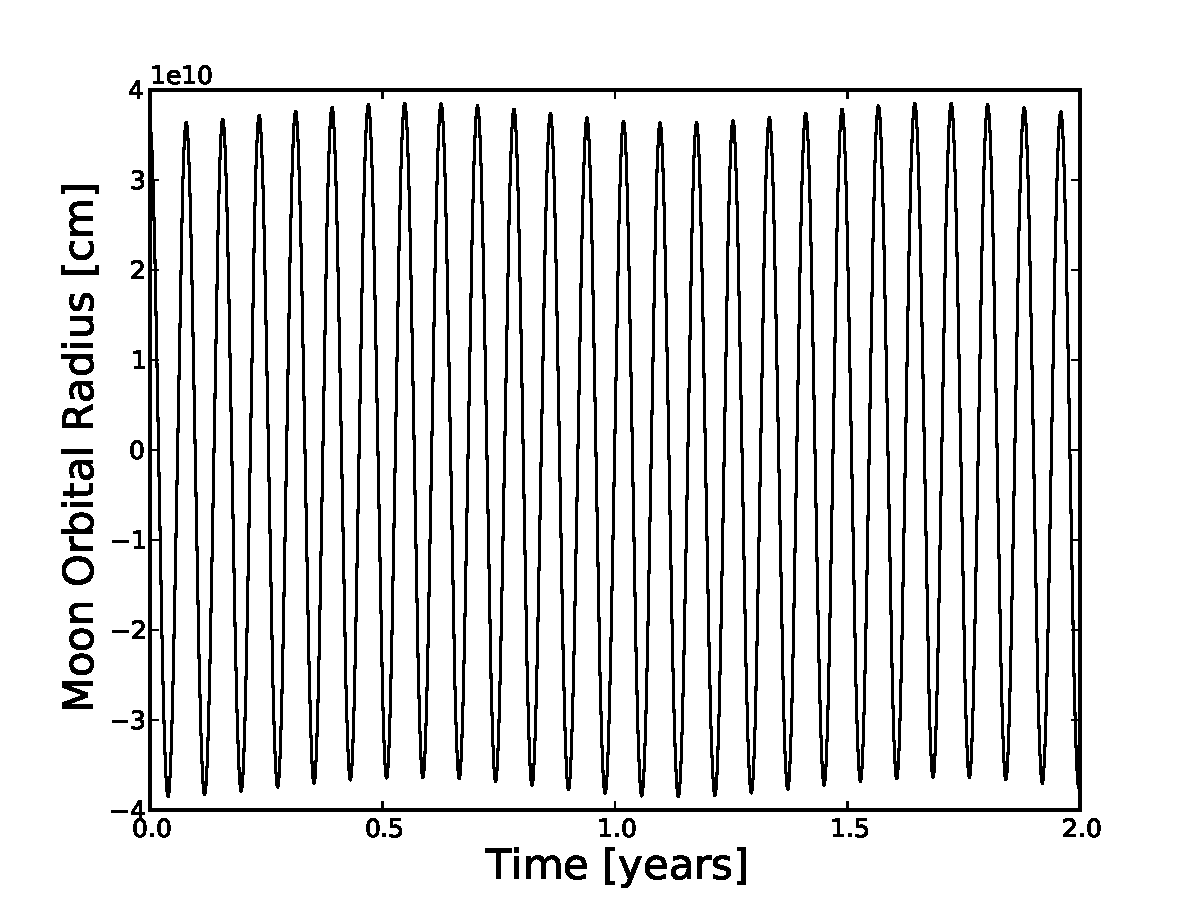
\includegraphics[width=0.7\textwidth]{moonorb.pdf}
\caption{Moon's orbital radius around Earth for two years. We get stability using only 3000 Nsteps and assuming no inclination.}
\label{fig:7}
\end{figure}

\begin{figure}[bth]
\centering
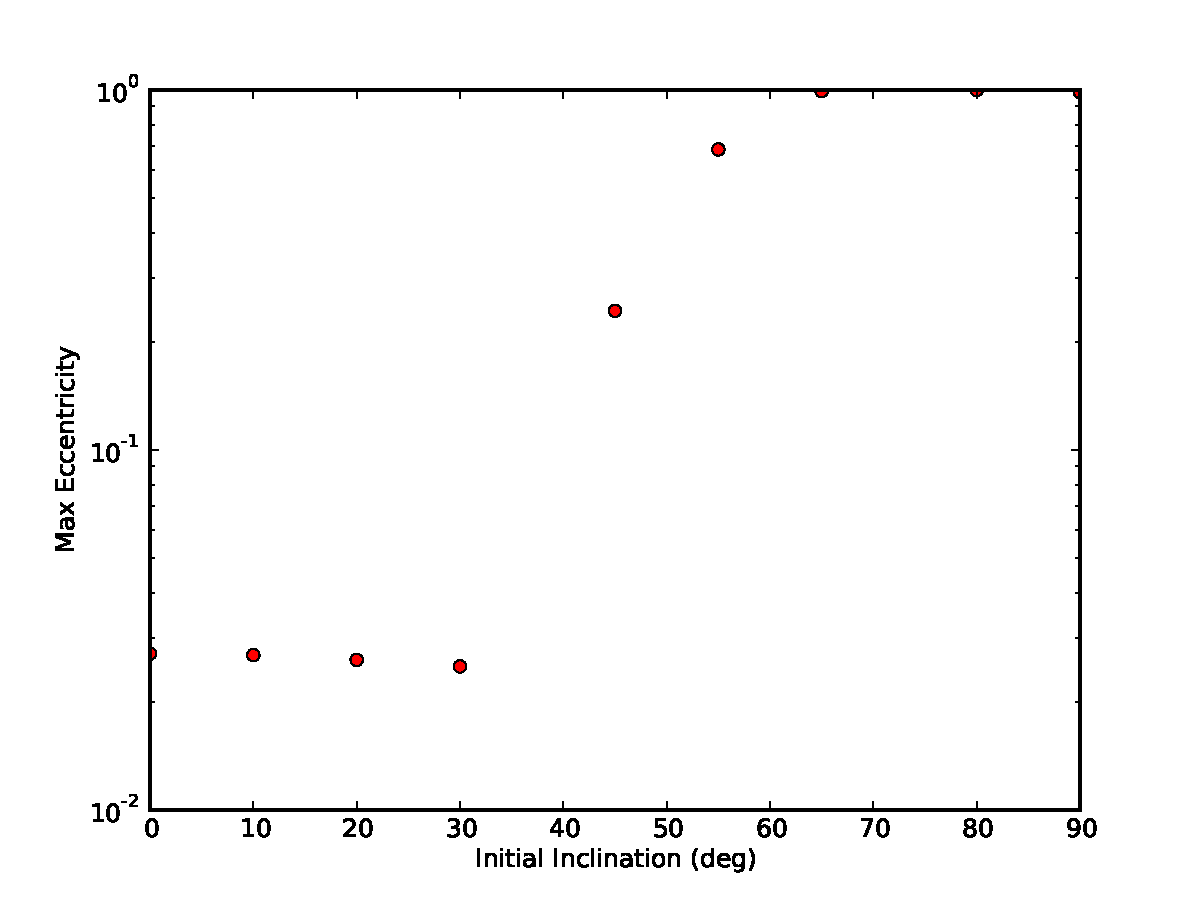
\includegraphics[width=0.7\textwidth]{ecc1.pdf}
\caption{The Kozai Mechanism for the Sun-Earth-Moon system. In our hierarchical 3-body system, we see the moon exchange of inclination for eccentricity over several orbits.}
\label{fig:8}
\end{figure}

\end{document}
